\documentclass[tikz,border=2pt]{standalone}
\usepackage{amsmath,amssymb}
\usepackage{tikz}
\usetikzlibrary{arrows.meta}

\begin{document}
% Composition: first B (U -> V), then A (V -> W); the product AB is one linear map U -> W,
% and its matrix is the matrix product.
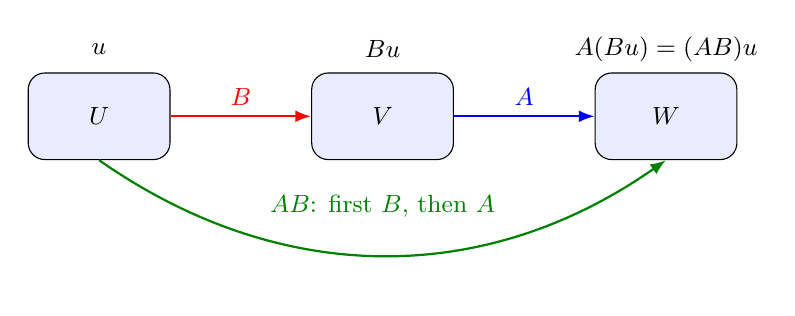
\begin{tikzpicture}[every node/.style={font=\small}, >={Latex[length=2mm]}]
	\node[draw, rounded corners=6pt, minimum width=1.8cm, minimum height=1.1cm, fill=blue!8] (U) at (0,0) {$U$};
	\node[draw, rounded corners=6pt, minimum width=1.8cm, minimum height=1.1cm, fill=blue!8] (V) at (3.6,0) {$V$};
	\node[draw, rounded corners=6pt, minimum width=1.8cm, minimum height=1.1cm, fill=blue!8] (W) at (7.2,0) {$W$};
	\draw[->, thick, red] (U) -- (V) node[midway, above] {$B$};
	\draw[->, thick, blue] (V) -- (W) node[midway, above] {$A$};
	\draw[->, thick, green!50!black] (U.south) to[bend right=35] node[midway, above=10pt] {$AB$: first $B$, then $A$} (W.south);
	\node[font=\small] at (0,0.85) {$u$};
	\node[font=\small] at (3.6,0.85) {$Bu$};
	\node[font=\small] at (7.2,0.85) {$A(Bu)=(AB)u$};
\end{tikzpicture}
\end{document}
